\documentclass[accentcolor=tud1b,colorbacktitle,inverttitle,landscape,presentation,t]{tudbeamer}
\usepackage[utf8]{inputenc}
\usepackage[german]{babel}
\usepackage{verbatim, hyperref,multimedia}
\usepackage{graphicx, psfrag}			%to insert graphics
\usepackage{setspace}
\usepackage[active]{srcltx}
\usepackage{color}
\usepackage{subfigure}
\usepackage{listings}
\usepackage{pstricks}
\usepackage{amssymb}

\useinnertheme{default}
\usecolortheme{orchid}
\setbeamercovered{transparent}


\newcommand{\keyword}[1]{\textcolor{tudaccent}{\textbf{#1}}} 
\newcommand{\myframetitle}[2]{\frametitle{#1 \\[.2cm] \small #2}}
\newcommand{\fatitem}[1]{\item \textbf{#1}}
\newcommand{\tab}{\hspace*{0.5cm}}


\setcounter{tocdepth}{1} 

\hypersetup{
pdftitle={WebMining Exercise }, pdfauthor={F. Englert}
}


\begin{document}

\title[MGA]{\large 4. Exercise}

\author{Frank Englert, Jens Haase}
\institute{KE, TU Darmstadt}

\logo{
\includegraphics{graphics/keico.eps}}

\date{May 2011}

\begin{titleframe}
\begin{center}
\color{tudtextaccent} \large Die 4. Übung\\[.5cm]
%\includegraphics[width=0.4\textwidth]{Graphics/spg_logo_final.eps} \\
\normalcolor \normalsize Knowlege Engineering \\
Fachbereich Informatik \\
Technische Universität Darmstadt\\[.5cm]

\textbf{Präsentation der Ergebnisse:}\\
Frank Englert\\ 
Jens Haase
\end{center}

\end{titleframe}  

\begin{frame}[c]
	\myframetitle{5. Übung}{Inhalt}

\end{frame}

\begin{frame}[c]
	\myframetitle{Task 1 - Language detection}{Language Detection via letter
	distribution}
\begin{itemize}
  \item The Firefox Plugin uses two detection modes
  \begin{itemize}
    \item Via letter frequency analysis
    \item Via syllable frequency analysis
  \end{itemize}
  \item The language detection algorithm is the same for both cases
  \item Advantages of using two detection modes:
  \begin{itemize}
    \item Double check the language detection results
    \item Collect information which mode works better
  \end{itemize}
  \item The Source of the frequency tables is http://bit.ly/jZHf0H
\end{itemize}
\end{frame}

\begin{frame}[c]
\myframetitle{Task 1 - Language detection}{Algorithm details}
\begin{itemize}
  \fatitem{The algorithms works with the following steps}
  \item A chunk is either a letter or a syllable
  \item dict contains the most important chunks of a language sorted by rank
\begin{enumerate}
  \item Take the text an split it to chunks(letters or syllables)
  \item Remove all chunks which are not in the dict
  \item Count the chunks and sort them by the count value. The result of this
  step is further called rankedChunks
  \item The weighted difference between the dictionary and the rankedChunks is
  \begin{itemize}
  \item $ \sum _{i=0}^{len(dic)} \frac{| i - rankedChunks.indexOf(dict[i]) |
  }{log _2 (i+2)}
  $
  \item If dict and rankedChunks are equals the weighted difference is 0
\end{itemize}
\end{enumerate}
\item repeat the steps 1-4 for all available languages. Take the language with
the lowest rank.
\end{itemize}
\end{frame}

\begin{frame}[c]
	\myframetitle{Task 1 - Language detection}{Letter frequency revisited}
\begin{figure}[htp]
\begin{center}
  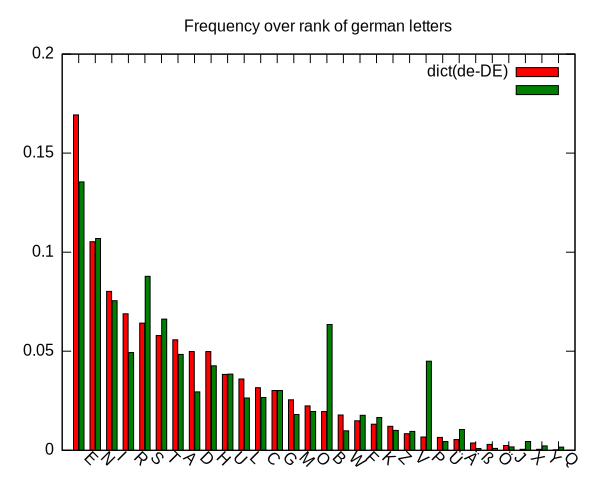
\includegraphics[width=1\textheight]{graphics/letters_de}
  \caption[fig:letters_de]{The frequency of german letters used
  for the Firefox plugin}
  \label{figureLabel}
\end{center}
\end{figure}

\end{frame}

\begin{frame}[c]
	\myframetitle{Task 1 - Language detection}{Syllable frequency revisited}

\begin{figure}[htp]
\begin{center}
  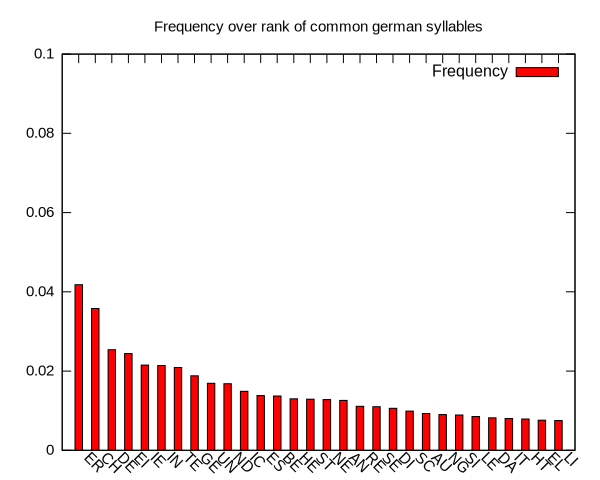
\includegraphics[width=1\textheight]{graphics/syllables_de}
  \caption[fig:letters_de]{The frequency of common german syllables used for the Firefox plugin}
  \label{figureLabel}
\end{center}
\end{figure}

\end{frame}


\begin{frame}[c]
	\myframetitle{Task 1 - Language detection}{Results of the language challenge}

\begin{table}
\begin{tabular}{|l|l|l|}
\hline
\textbf{Rank} &\textbf{letter lang}&\textbf{syllable lang}\\
\hline
1 &englisch&-\\
2 &englisch&-\\
3&deutsch&-\\
4&französisch&-\\
5&deutsch&-\\
6&deutsch&deutsch\\
7&französisch&französisch\\
8&französisch&französisch\\
9&englisch&englisch\\
10&deutsch&deutsch\\
\hline
\end{tabular}
\caption{Detection results of the firefox plugin}
\label{tablelabel}
\end{table}

\end{frame}

\begin{frame}[c]
	\myframetitle{Task 1 - Language detection}{Further improvement}
	
	\begin{itemize}
	\fatitem{Easy:}
	\begin{itemize}
		\item Add more languages
	\end{itemize}
	
	  \fatitem{A lot of work:}
	  \begin{itemize}
  	    \item The Plugin checks already p, div and span tags. It would be better
  	  to check the text content of all tags.
  	    \item Try to estimate the best detection result if the syllable and the
  	letter mode returns different results
      \end{itemize}
      \fatitem{Most Interesting:}
      \begin{itemize}
  		\item Improve the weighting algorithm to reduce the amount of needed text
  		\item Implement a learning mode to train new languages

	\end{itemize}
	\end{itemize}
\end{frame}
\begin{frame}[c]
  \myframetitle{Aufgabe 2}{Suche mittels HITS}
\begin{itemize}
  \item Berechnet die Wahrscheinlichkeit das eine Seite ein Hub oder eine Authority ist
  \item Muss bei jeder Suchanfrage neu berechnet werden
  \item In der Übung wurde die Iterative Methode verwendet
  \item Der Algorithmus terminiert meistens nach 11 Iterationen
\end{itemize}
\end{frame}

\begin{frame}[c]
    \myframetitle{HITS}{Authority ist hoch bei vielen eingehenden Links}
    %\usepackage{graphics} is needed for \includegraphics
\begin{figure}[htp]
\begin{center}
  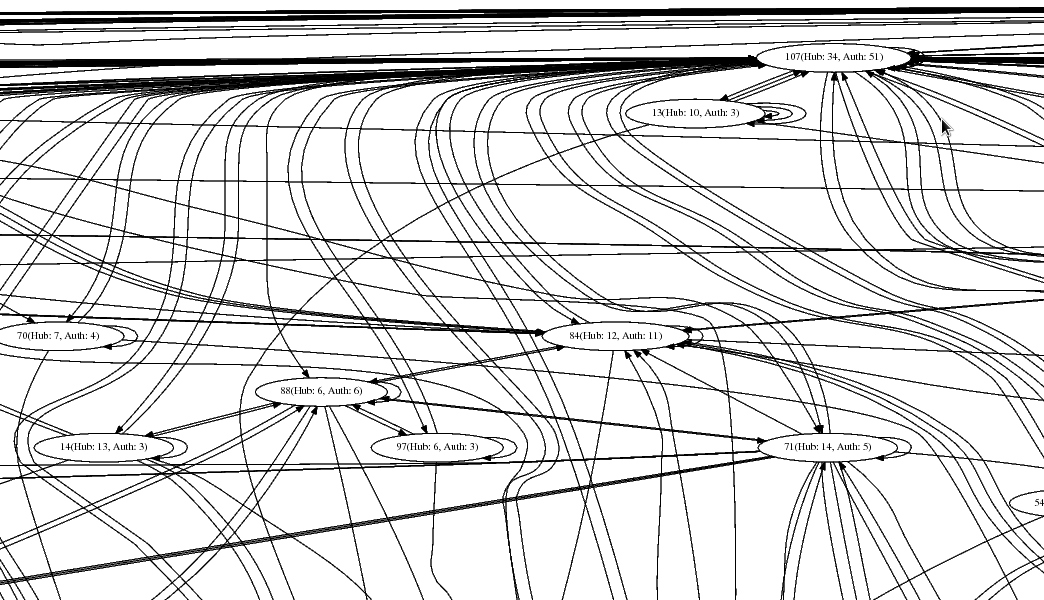
\includegraphics[height=1\textheight]{graphics/hitsGraph.png}
%  \caption[labelInTOC]{}
%  \label{fig:hihg_inoutdegree}
\end{center}
\end{figure}

\end{frame}
\begin{frame}[c]
  \myframetitle{Aufgabe 2}{Suche mittels Page-Rank}
\begin{itemize}
  \fatitem{Der Page-Rank ist die Wahrscheinlichkeit eines Websiten-Besuchs}
  \item Das Ranking der Websites kann offline erfolgen
  \item Für die Übung wurde das Iterative Pagerank-Verfahren implementiert
  \item Der Algorithmus konvergiert nach 30 Iterationen auf dem Beispielgraph
\end{itemize}
\end{frame}

\begin{frame}[c]
\myframetitle{Page-Rank}{Verteilung des Page-Ranks}
%\usepackage{graphics} is needed for \includegraphics
\begin{figure}[htp]
\begin{center}
  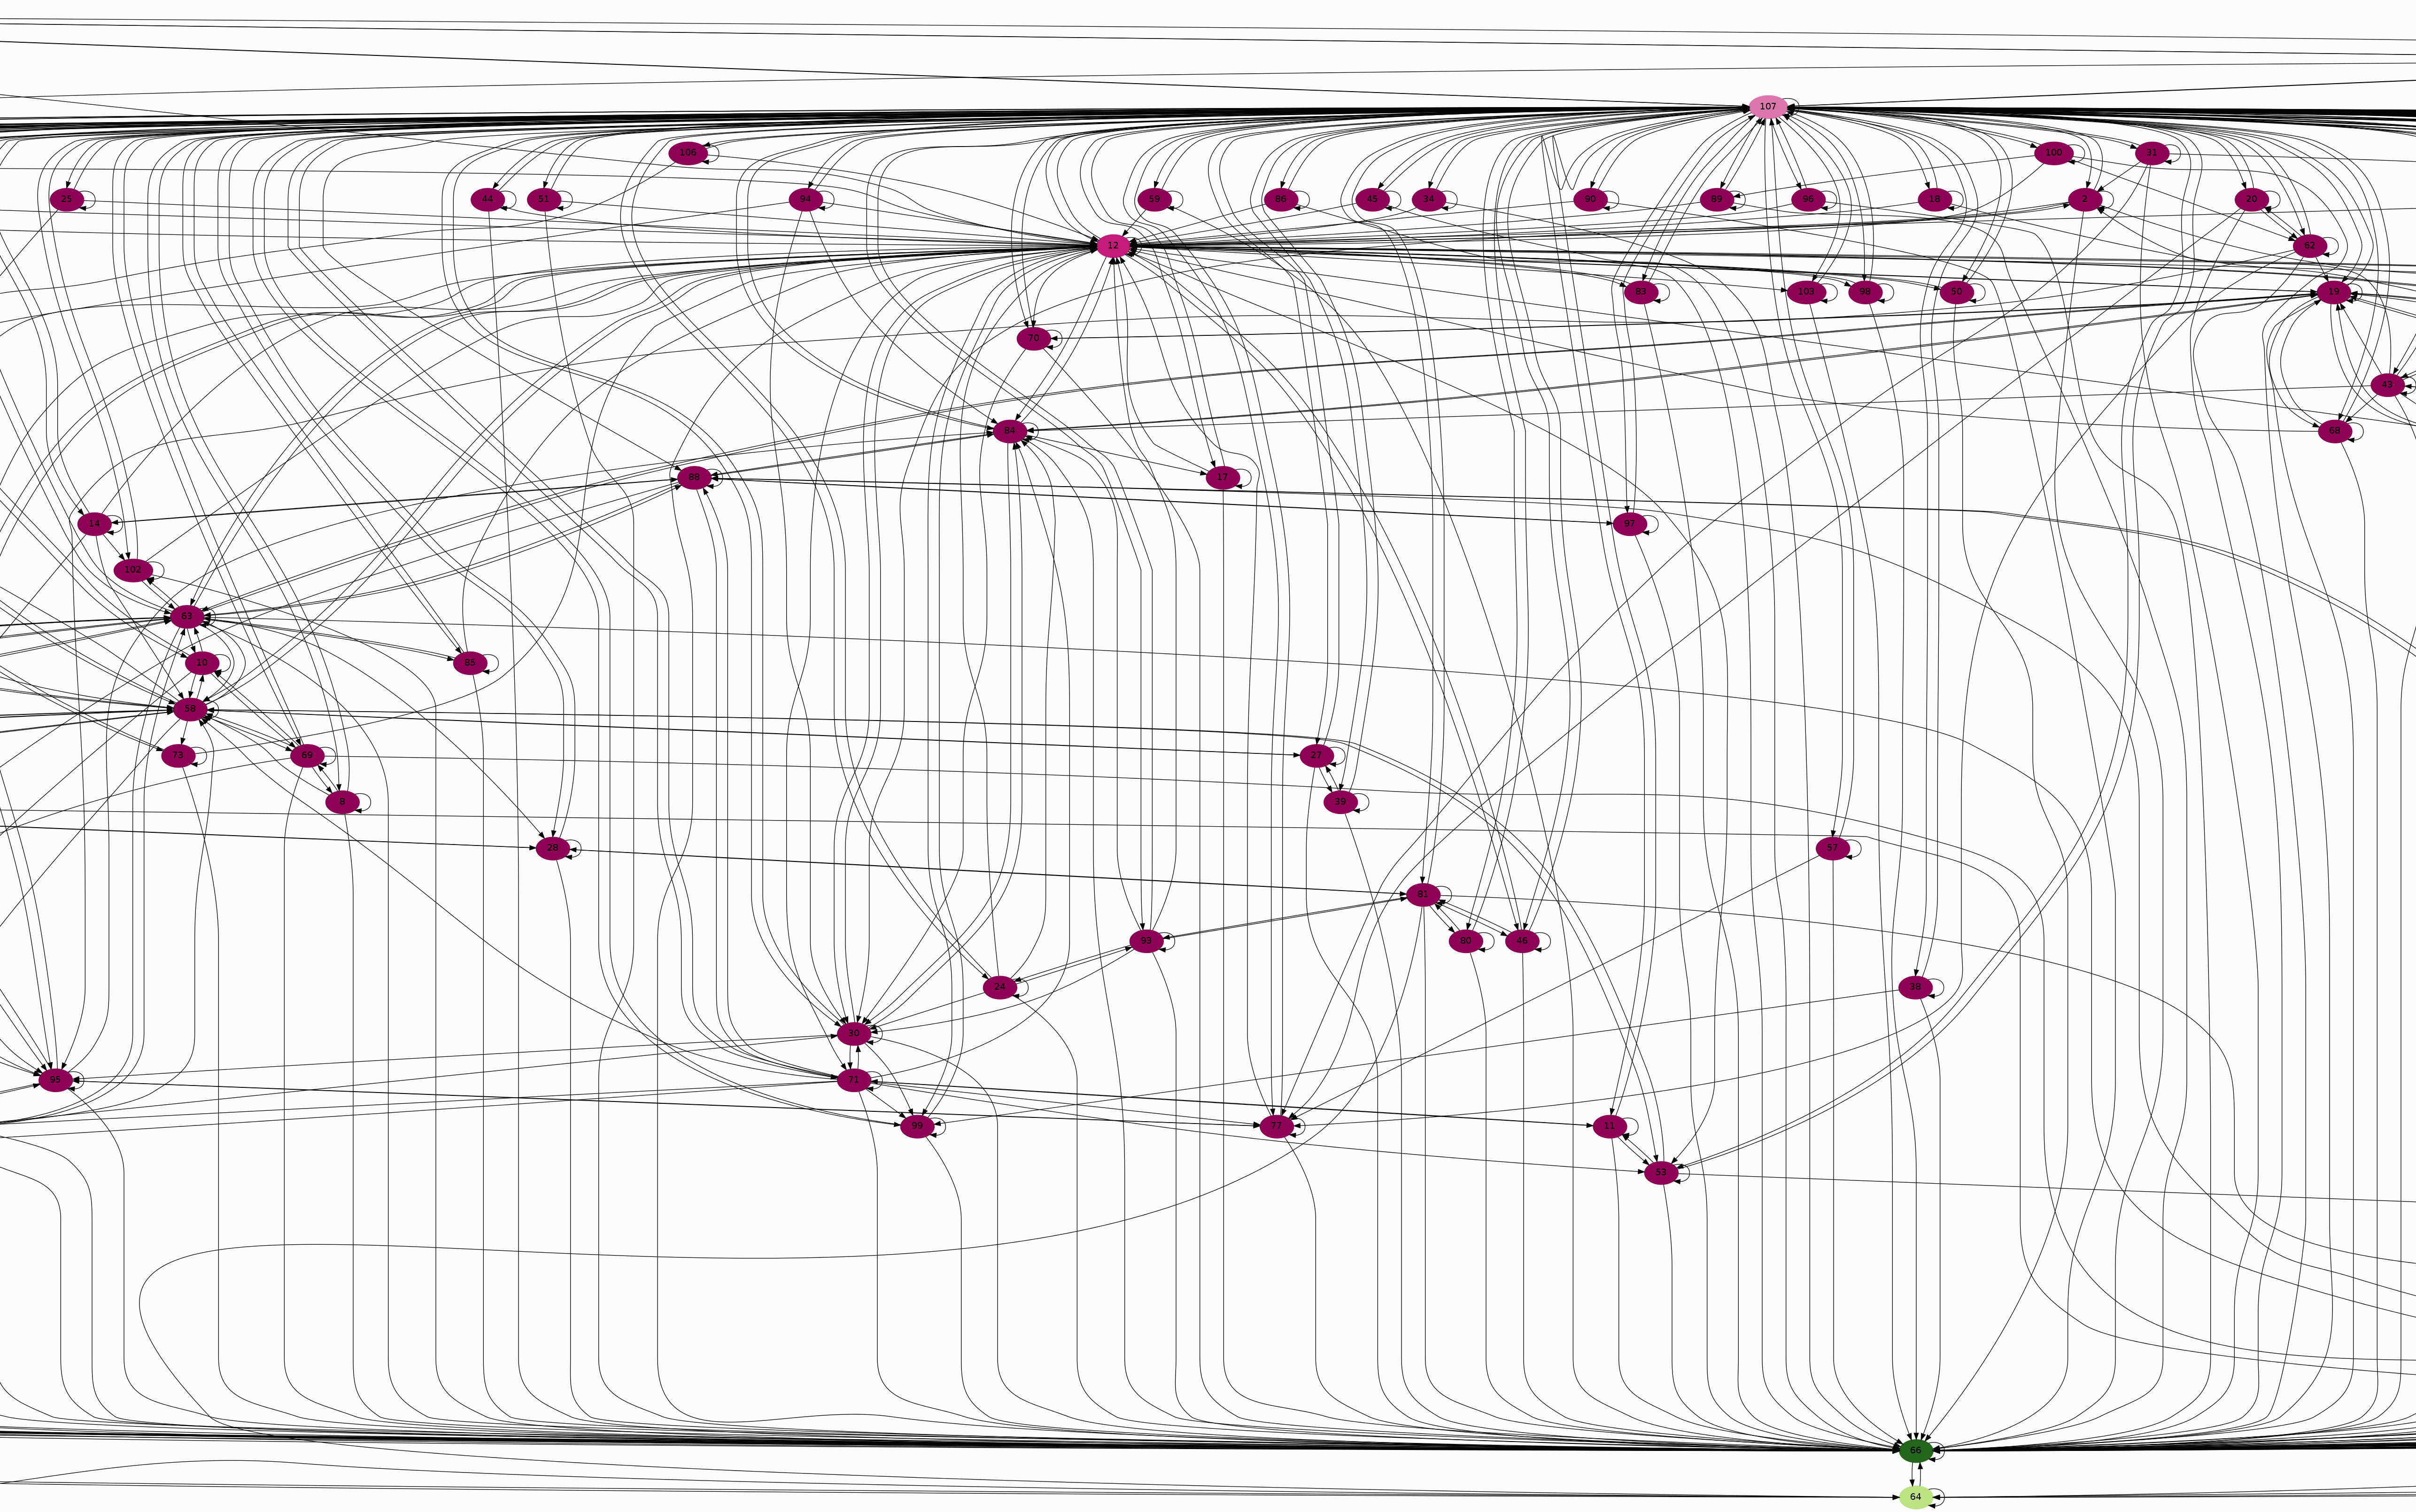
\includegraphics[height=1\textheight]{graphics/pr_overview.png}
  \caption[labelInTOC]{}
  \label{fig:prOverview} 
\end{center}
\end{figure}
\end{frame}

\begin{frame}[c]
    \myframetitle{Page-Rank}{PR ist hoch bei hohem In-Degree}
    %\usepackage{graphics} is needed for \includegraphics
\begin{figure}[htp]
\begin{center}
  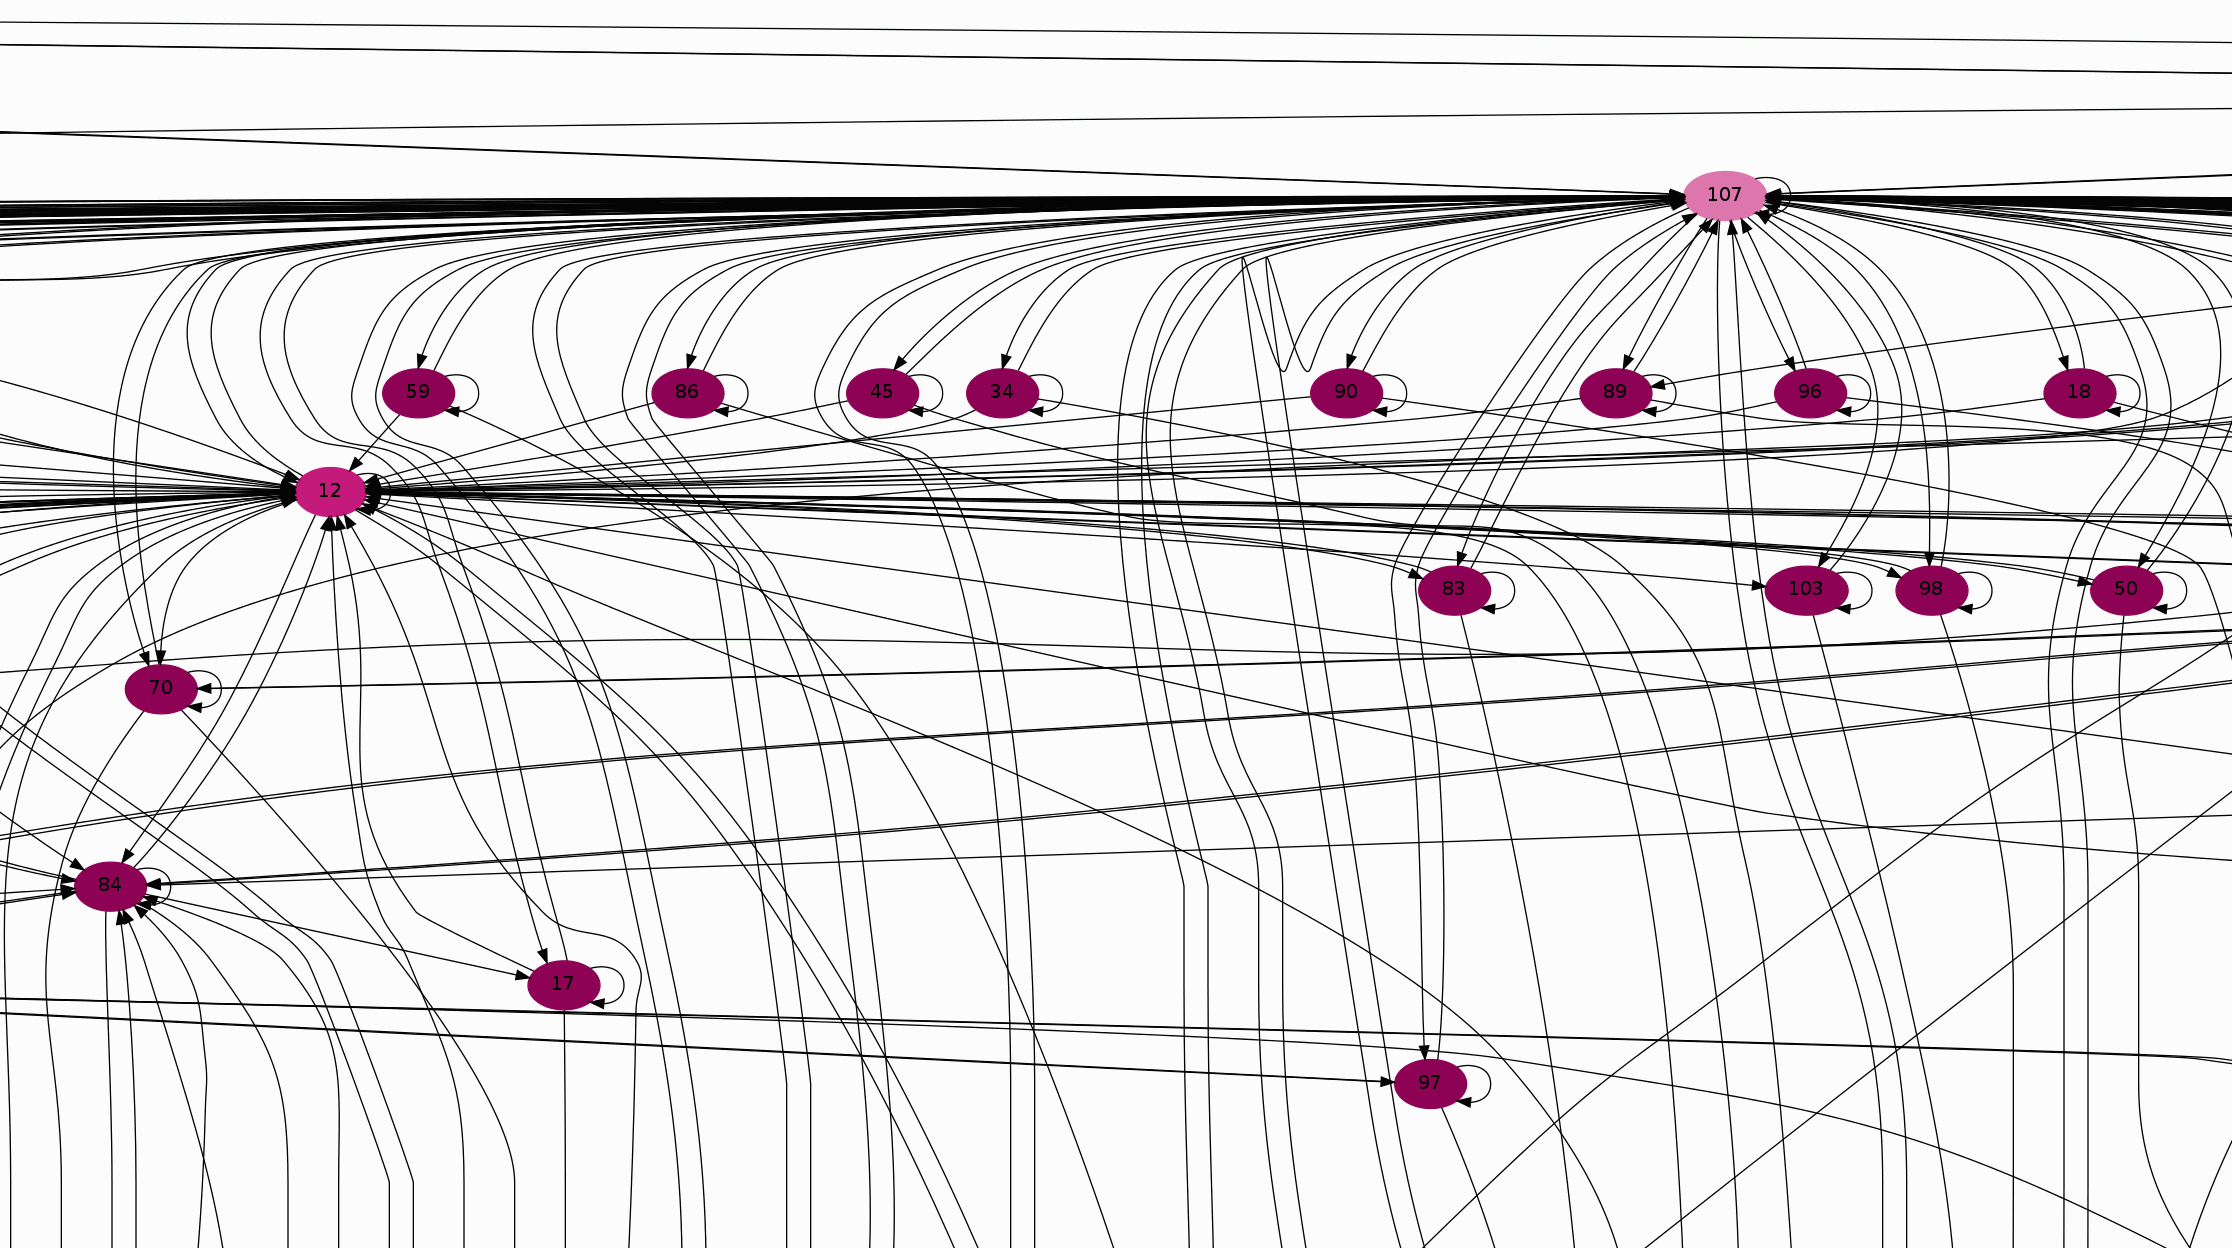
\includegraphics[height=1\textheight]{graphics/pr_high_inout_degree.png}
%  \caption[labelInTOC]{}
%  \label{fig:hihg_inoutdegree}
\end{center}
\end{figure}

\end{frame}


\begin{frame}[c]
    \myframetitle{Page-Rank}{PR ist hoch bei kleinem Out-Degree der Vorgänger}
%\usepackage{graphics} is needed for \includegraphics
\begin{figure}[htp]
\begin{center}
  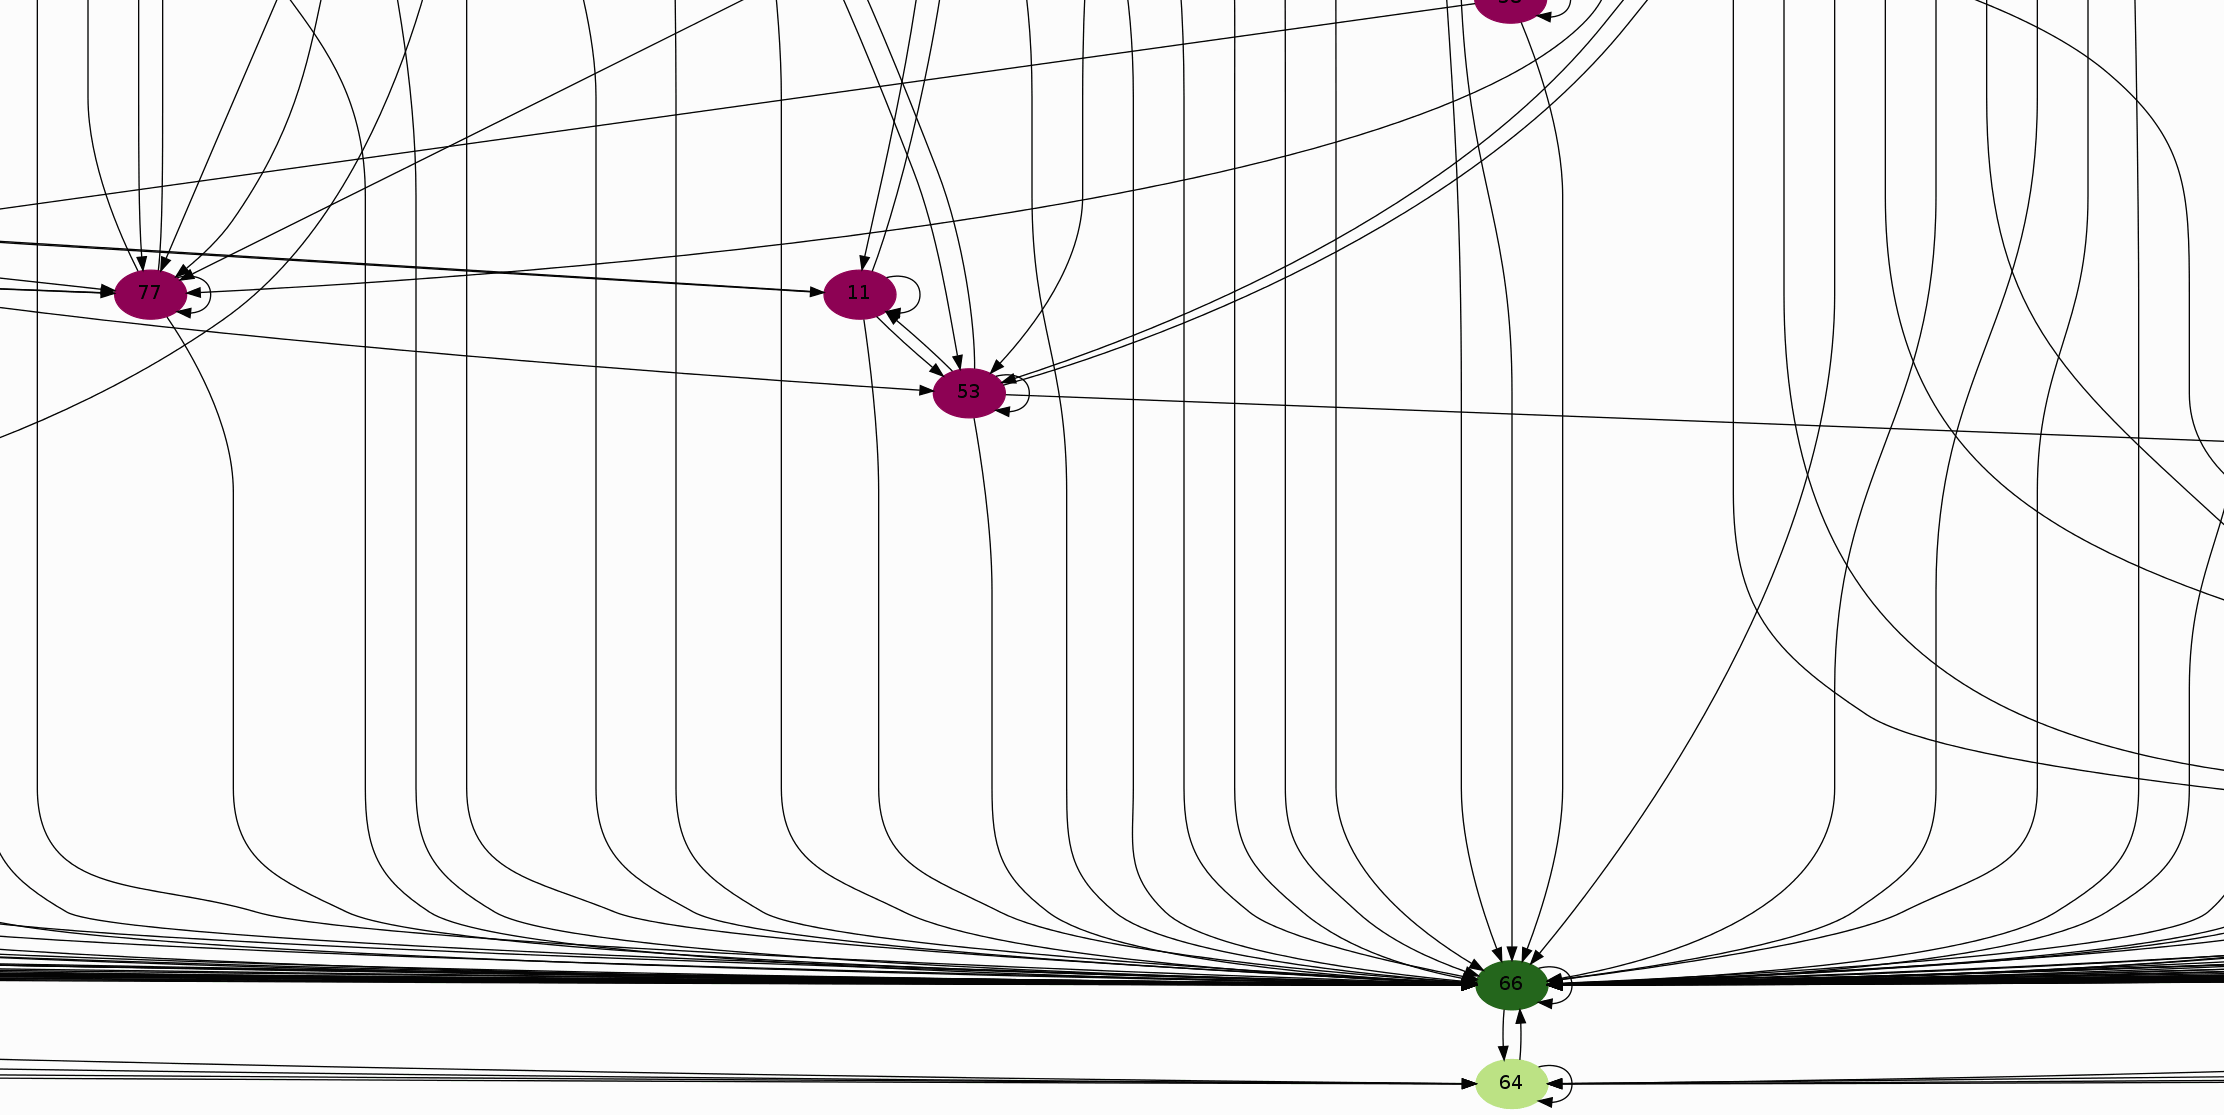
\includegraphics[height=1\textheight]{graphics/high_indegree.png}
%  \caption[labelInTOC]{}
%  \label{fig:prHighIndegree}
\end{center}
\end{figure}
\end{frame}

\begin{frame}[c]
    \myframetitle{Page-Rank}{Ranking des Graphen aus Aufgabe 1}
    \begin{itemize}
  \fatitem{Für den Graph aus Aufgabe 1 ergibt sich folgendes Ranking:}
\begin{enumerate}
  \item ID(66)	PR(0,28804), Special Categories
  \item ID(64)	PR(0,22126), Wikipedia Categorization
  \item ID(107) PR(0,06453), Category Data mining
  \item ID(12)	PR(0,03134), Data mining
  \item ID(91)	PR(0,01396), Why  might a category list\ldots
  \item ID(58)	PR(0,01061), Cluster analysis
\end{enumerate}
\ldots
\begin{enumerate}[100.]
\item  ID(104)	PR(0,00223), Affinity analysis
\end{enumerate}
\item Max(PR)=0,28804 Min(PR)=0.00223
\item Die Wahrscheinlichkeit durch zufälliges Surfen auf die Seite
``Special Categories'' zu kommen beträgt demnach 28\%
\item Die Wahrscheinlichkeit durch zufälliges Surfen auf ``Affinity Analysis'' zu
kommen beträgt nur 0.2\%
\end{itemize}
\end{frame}


\end{document}
